\documentclass{article}
\usepackage{graphicx} % Required for inserting images
\usepackage{listings}
\usepackage{xcolor}

\title{Assignment 3 report}
\author{Yisi Liu}
\date{March 2024}

%New colors defined below
\definecolor{codegreen}{rgb}{0,0.6,0}
\definecolor{codegray}{rgb}{0.5,0.5,0.5}
\definecolor{codepurple}{rgb}{0.58,0,0.82}
\definecolor{backcolour}{rgb}{0.95,0.95,0.92}

%Code listing style named "mystyle"
\lstdefinestyle{mystyle}{
  backgroundcolor=\color{backcolour},   commentstyle=\color{codegreen},
  keywordstyle=\color{magenta},
  numberstyle=\tiny\color{codegray},
  stringstyle=\color{codepurple},
  basicstyle=\ttfamily\footnotesize,
  breakatwhitespace=false,         
  breaklines=true,                 
  captionpos=b,                    
  keepspaces=true,                 
  numbers=left,                    
  numbersep=5pt,                  
  showspaces=false,                
  showstringspaces=false,
  showtabs=false,                  
  tabsize=2
}

\lstset{style=mystyle}

\begin{document}

\maketitle

\section{Introduction}

Linear algebra, matrices, and the ability to work with them through 2D arrays in C are very useful skills, which was practiced in this assignment. In this report, I will explain Gaussian Elimination, which I used as the algorithm for solving linear systems of equations in the form of Ax = B where A and B are given. I will also explain why my code crashes with a segmentation fault when typing ``./math\_matrix.c 512 512 512 512 add'' in the terminal. Finally, my complete codes are attached in Appendix 1. 

\section{The Algorithm}

Ax = B is one way to represent a linear system of equations, and one very code-friendly, algorithmic way to solve it is by taking the column vector B, augmenting A with it, and row-reducing the resulting matrix. The answer will be the final column. 

To row-reduce, first, divide the first row by the first number in the row to get a leading 1 in the first column of the first row. Then, add the appropriate multiple of the first row to all subsequent rows so that everything in the first column below the leading 1 sum to a zero. This appropriate multiple will be the negative of the first entry of the row in question. 

Next, repeat the same steps except with the second entry of the second number. 

Repeat until the final row is reached. This will reach the second-last column because A must be square to ensure a unique solution, and B is a column vector. 

The so-called backwards phase then begins, where appropriate multiples of rows are added to the rows above them to turn everything in a column with a leading 1, other than said leading 1, into a zero. The appropriate multiple is, again, the negative of the entry in the same column as the specific column being cleared for whichever row being added to at any given time. 

Once the augmented matrix resembles an identity matrix with a random column vector stuck to its right side, that last column will be x.

\section{Segmentation fault}

A segmentation fault occurs when attempting to run ``./math\_matrix.c 512 512 512 512 add'' in terminal, but not right before.
\\

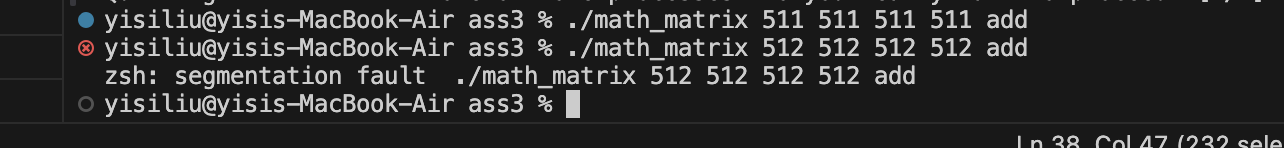
\includegraphics[width = 12cm]{terminal.png}
\\

Any number bigger than 512 also produces the same error in my computer. 

This is because this segmentation fault is caused by stack overflow, just like the example shown in lecture of trying to create an array \\``int largeArray[2098100]'' within the main() function because what that does is that it's asking for memory. It asks to be allocated the space in memory to store an integer array of size 2098100, and since it is a local variable because it's within the main() function, it's allocated memory in the stack where information about function calls, including local variables, are stored, automatically. The stack has a set, restricted size, however, and exceeding that size (a stack overflow)counts as assessing illegal memory, which is a segmentation fault. 

Within my code, I first automatically allocate on stack ``double A[512][512]'', then ``double B[512][512]'', then simultaneously ``resultadd[512][512]'' and ``resultx[512][512]'' both doubles. The sum of the space in memory I'm asking for just exceeds ('cause 511 is still within limits)my system specifications (someone else's system specifications may allow up to 591, or anything else)for the stack size and I produce a segmentation fault due to stack overflow. 

This is clearly evident when stepping through my code with lldb, and seeing that the second I hit the line with resultadd and resultx, the error appears because that is the line where everything together finally exceeds the limit of my stack. 
\\
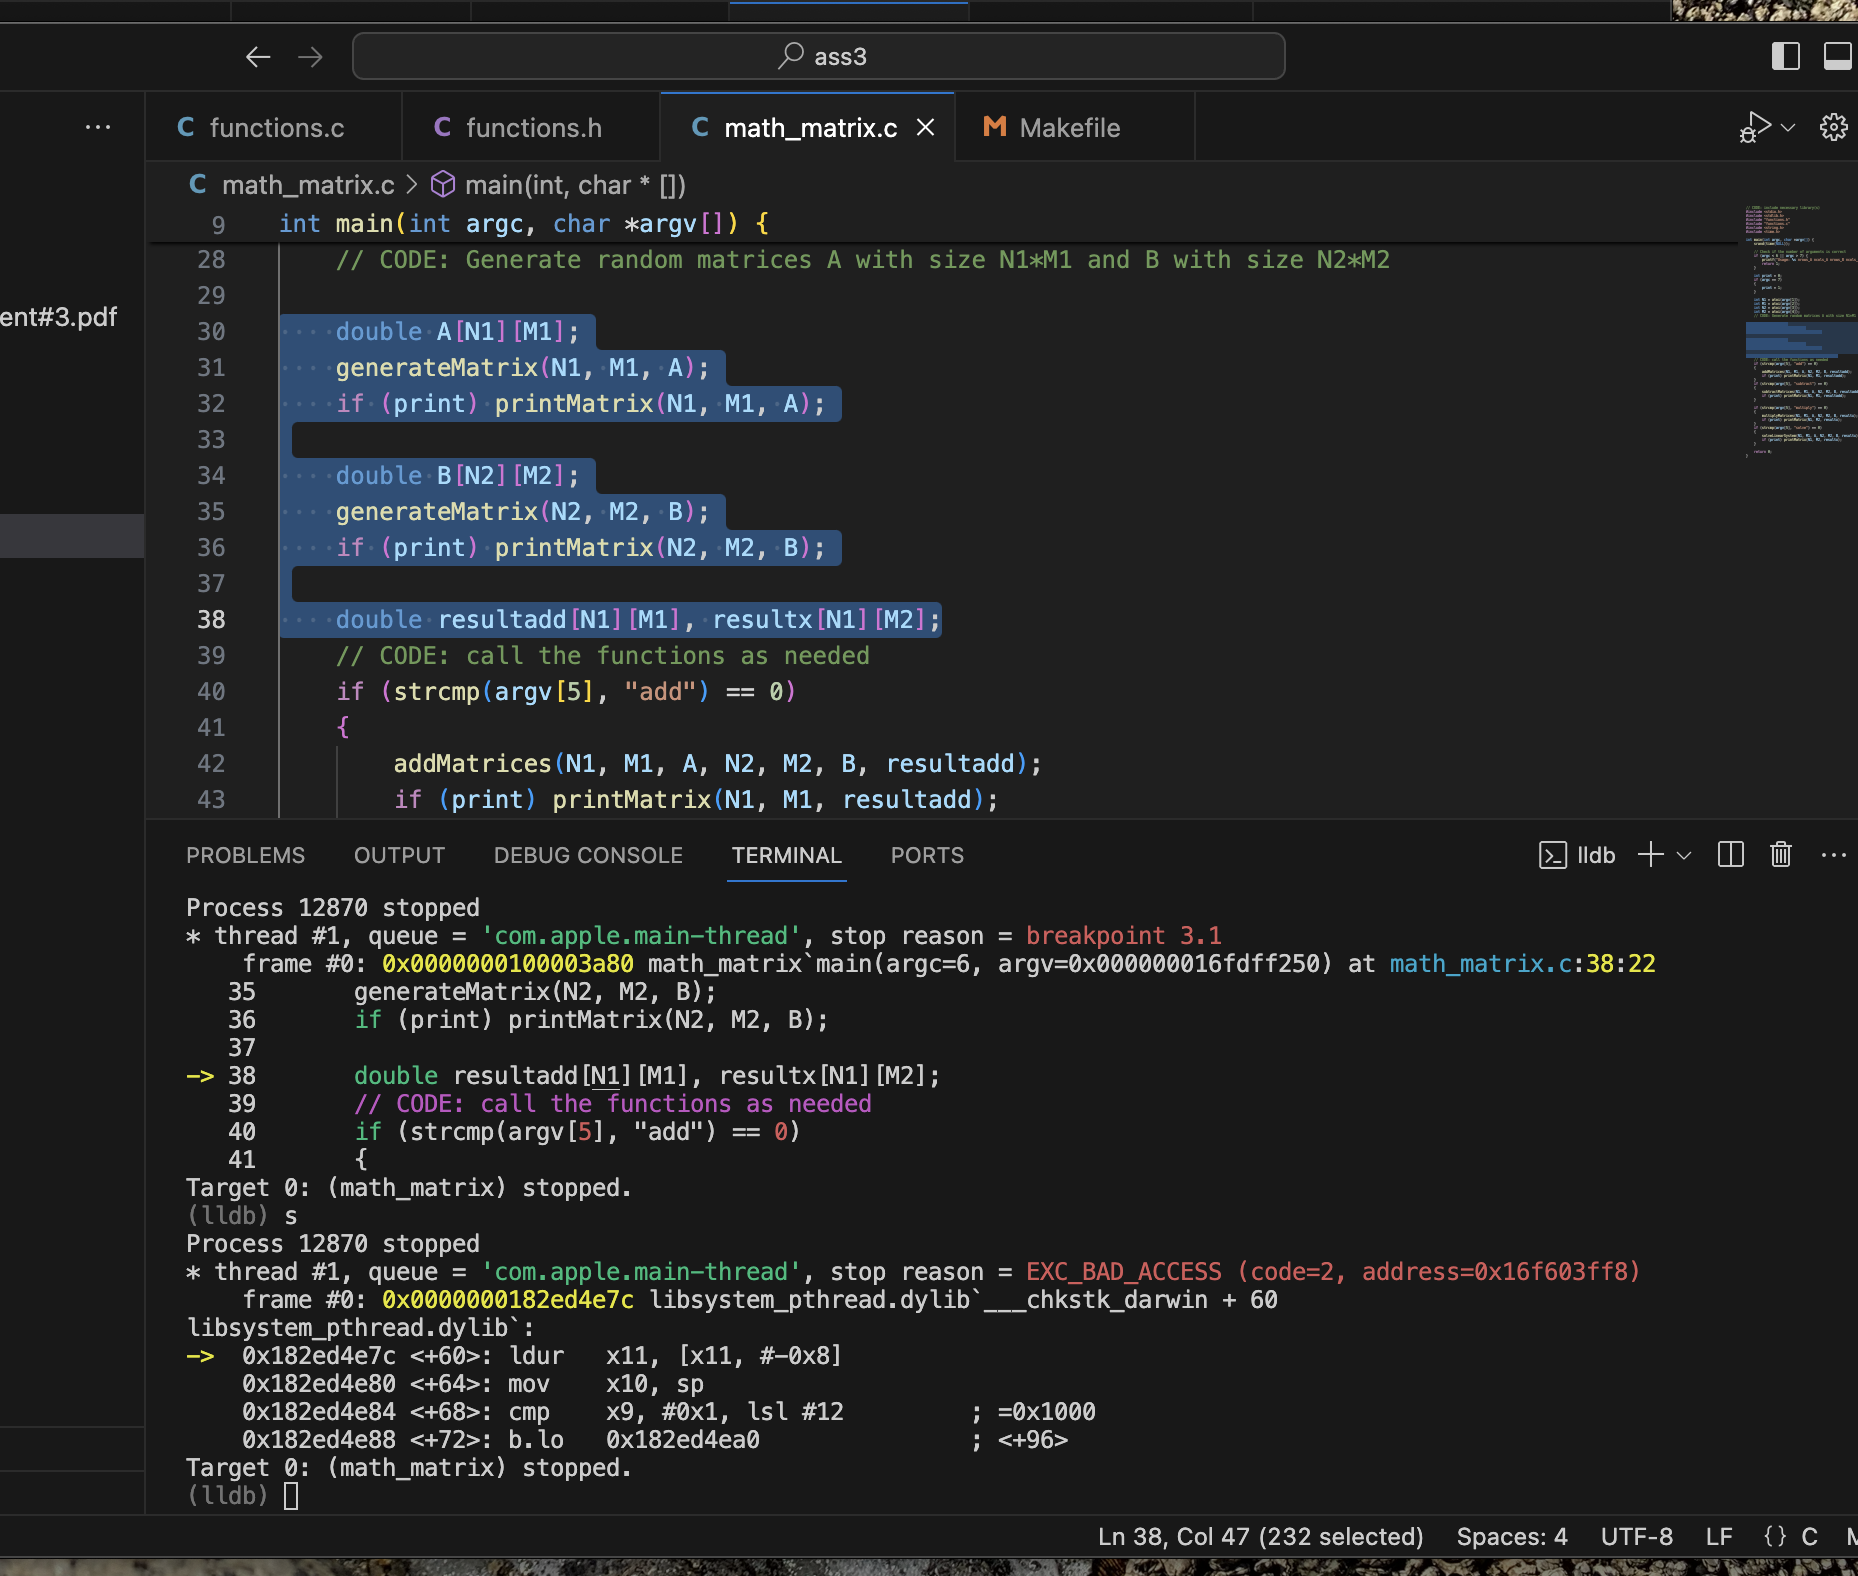
\includegraphics[width = 12cm]{lldb.png}
\\
\\
\section{Appendix 1}

The following are my complete code files. 

\begin{lstlisting}[language=C, caption=math\_matrix.c]
// CODE: include necessary library(s)
#include <stdio.h>
#include <stdlib.h>
#include "functions.h"
#include "functions.c"
#include <string.h>
#include <time.h>

int main(int argc, char *argv[]) {
    srand(time(NULL));

    // Check if the number of arguments is correct
    if (argc < 6 || argc > 7) {
        printf("Usage: %s nrows_A ncols_A nrows_B ncols_B <operation> [print]\n", argv[0]);
        return 1;
    }

    int print = 0;
    if (argc == 7)
    {
        print = 1;
    }

    int N1 = atoi(argv[1]);
    int M1 = atoi(argv[2]);
    int N2 = atoi(argv[3]);
    int M2 = atoi(argv[4]);
    // CODE: Generate random matrices A with size N1*M1 and B with size N2*M2
    
    double A[N1][M1];
    generateMatrix(N1, M1, A);
    if (print) printMatrix(N1, M1, A);

    double B[N2][M2];
    generateMatrix(N2, M2, B);
    if (print) printMatrix(N2, M2, B);

    double resultadd[N1][M1], resultx[N1][M2];
    // CODE: call the functions as needed
    if (strcmp(argv[5], "add") == 0)
    {
        addMatrices(N1, M1, A, N2, M2, B, resultadd);
        if (print) printMatrix(N1, M1, resultadd);
    }
    if (strcmp(argv[5], "subtract") == 0)
    {
        subtractMatrices(N1, M1, A, N2, M2, B, resultadd);
        if (print) printMatrix(N1, M1, resultadd);
    }

    if (strcmp(argv[5], "multiply") == 0)
    {
        multiplyMatrices(N1, M1, A, N2, M2, B, resultx);
        if (print) printMatrix(N1, M2, resultx);
    }
    if (strcmp(argv[5], "solve") == 0)
    {
        solveLinearSystem(N1, M1, A, N2, M2, B, resultx);
        if (print) printMatrix(N1, M2, resultx);
    }

    return 0;
}
\end{lstlisting}

\begin{lstlisting}[language=C, caption=functions.c]
// CODE: include necessary library(s)
#include <stdio.h>
#include <stdlib.h>
#include "functions.h"

// Function to generate a random matrix
void generateMatrix(int rows, int cols, double matrix[rows][cols]) {
    // CODE: Generate random numbers between -10 and 10

    for (int i = 0; i < rows; i++)
    {
        for (int j = 0; j < cols; j++)
        {
            matrix[i][j] = (rand()%20000000)/(double)1000000 - 10;
        }
    }
}

// Function to print a matrix
void printMatrix(int rows, int cols, double matrix[rows][cols]) {
    // CODE: to print the matrix 

    for (int i = 0; i < rows; i++)
    {
        for (int j = 0; j < cols; j++)
        {
            printf("%lf ", matrix[i][j]);
        }
        printf("\n");
    }
    printf("\n");
}

// Function to add two matrices
void addMatrices(int N1, int M1, double A[N1][M1], int N2, int M2, double B[N2][M2], double result[N1][M1]) 
{   // CODE: check for the condition 
    if (N1 != N2 || M1 != M2)
    {
        printf("Matrix sizes incompatible for addition. Result matrix will be random numbers or a system default.\n");
        return;
    }
    
    for (int i = 0; i < N1; i++)
    {
        for (int j = 0; j < M1; j++)
        {
            result[i][j] = A[i][j] + B[i][j];
        }
    }
}

void subtractMatrices(int N1, int M1, double A[N1][M1], int N2, int M2, double B[N2][M2], double result[N1][M1])
{   // CODE: check for the condition 
    if (N1 != N2 || M1 != M2)
    {
        printf("Matrix sizes incompatible for subtraction. Result matrix will be random numbers or a system default.\n");
        return;
    }
    
    for (int i = 0; i < N1; i++)
    {
        for (int j = 0; j < M1; j++)
        {
            result[i][j] = A[i][j] - B[i][j];
        }
    }
}

void multiplyMatrices(int N1, int M1, double A[N1][M1], int N2, int M2, double B[N2][M2], double result[N1][M2])
{
    if (M1 !=  N2)
    {
        printf("Matrix sizes incompatible for multiplication. Result matrix will be random numbers or a system default.\n");
        return;
    }
    
    for (int i = 0; i < N1; i++)
    {
        for (int j = 0; j < M2; j++)
        {
            double sum = 0;
            for (int k = 0; k < M1; k++)
            {
                sum += (A[i][k] * B[k][j]);
            }
            result[i][j] = sum;
        }
    }    

}

//creating forward-declared helper functions for row operations seperately to keep organized:
void interchange(int rows, int cols, double matrix[rows][cols], int idx1, int idx2);

void multiply(int rows, int cols, double matrix[rows][cols], int idx, double constant);

void addrow(int rows, int cols, double matrix[rows][cols], int idx1, int idx2, double constant);

void solveLinearSystem(int N1, int M1, double A[N1][M1], int N2, int M2, double B[N2][M2], double x[N1][M2])
{
    if (N1 != N2 || M2 != 1 || M1 != N1) //if A isn't square then there is no unique solution
    {
        printf("Matrix sizes incompatible for obtaining a solution for a linear system. Result matrix will be random numbers or a system default.\n");
        return;
    }

    double aug[N1][M1+1]; //augmenting A with B
    for (int i = 0; i < N1; i++)
    {
        for (int j = 0; j < M1; j++)
        {
            aug[i][j] = A[i][j];
        }
    }    
    for (int i = 0; i < N2; i++)
    {
        aug[i][M1] = B[i][0];//actual index of the last extra row is M1 + 1 - 1
    }
     
    for (int i = 0; i < N1; i++)//essentially iterating down the diagonal of A since it's square to perform Gaussian Elimination on the augmented matrix where B tags along
    {    
        multiply(N1, (M1+1), aug, i, (1/aug[i][i]));
        for (int j = i+1; j < M1; j++)
        {
            addrow(N1, (M1+1), aug, i, j, (-aug[j][i]));
        }
        
    }
    
    for (int i = (N1 - 1); i >= 0; i--)//now for the backwards phase
    {
        for (int j = i-1; j >= 0; j--)
        {
            addrow(N1, (M1+1), aug, i, j, (-aug[j][i]));
        }   
    }
    
    for (int i = 0; i < N2; i++)//the last column that tagged along is now the answer
    {
        x[i][0] = aug[i][M1];
    }     
}

void interchange(int rows, int cols, double matrix[rows][cols], int idx1, int idx2)
{
    double spare[cols];

    for (int j = 0; j < cols; j++)
    {
        spare[j] = matrix[idx2][j];
    }

    for (int j = 0; j < cols; j++)
    {
        matrix[idx2][j] = matrix[idx1][j];
    }
    
    for (int j = 0; j < cols; j++)
    {
        matrix[idx2][j] = spare[j];
    }
}

void multiply(int rows, int cols, double matrix[rows][cols], int idx, double constant)
{
    for (int j = 0; j < cols; j++)
    {
        matrix[idx][j] = (matrix[idx][j])*constant;
    }
}

void addrow(int rows, int cols, double matrix[rows][cols], int idx1, int idx2, double constant)
{
    for (int j = 0; j < cols; j++)
    {
        matrix[idx2][j] += (matrix[idx1][j])*constant;
    }
}
\end{lstlisting}

\end{document}



